\documentclass{article}
\usepackage[a4paper, hmargin={2.5cm, 2.5cm}, vmargin={2.5cm, 2.5cm}]{geometry}
\usepackage[utf8]{inputenc}
\usepackage[english]{babel}
\usepackage{amsmath,amssymb,graphicx}
\usepackage{cleveref}
\usepackage{hyperref}

\usepackage{mathtools}
\usepackage{fancyhdr}
\usepackage{lastpage}
\usepackage{geometry}
\usepackage{ulem}
\usepackage{gauss}
\usepackage{graphicx}
\usepackage{pdfpages}
\usepackage{hyperref}
\usepackage{cleveref}
\usepackage{wrapfig}
\usepackage{morefloats}
\usepackage{upquote}


%%%%%% COLORS %%%%%%%%

\usepackage{xcolor}
\definecolor{red1}{rgb}{0.7, 0.0, 0.3}
\definecolor{red2}{rgb}{0.5, 0.0, 0.5}
\definecolor{red3}{rgb}{0.3, 0.0, 0.7}

%two definitions of the color grey
\usepackage{color}
\definecolor{listinggray}{gray}{0.9}
%\definecolor{lbcolor}{rgb}{0.9,0.9,0.9}

\usepackage{listings}
\lstset{
	language=,
	literate=
		{æ}{{\ae}}1
		{ø}{{\o}}1
		{å}{{\aa}}1
		{Æ}{{\AE}}1
		{Ø}{{\O}}1
		{Å}{{\AA}}1
		{'}{{'}}1,
	backgroundcolor=\color{listinggray},
	tabsize=3,
	rulecolor=,
	basicstyle=\scriptsize,
	upquote=true,
	aboveskip={1.5\baselineskip},
	columns=fixed,
	showstringspaces=false,
	extendedchars=true,
	breaklines=true,
	prebreak =\raisebox{0ex}[0ex][0ex]{\ensuremath{\hookleftarrow}},
	frame=single,
	showtabs=false,
	showspaces=false,
	showstringspaces=false,
	identifierstyle=\ttfamily,
	keywordstyle=\color[rgb]{0,0,1},
	commentstyle=\color[rgb]{0.133,0.545,0.133},
	stringstyle=\color[rgb]{0.627,0.126,0.941},
}

\lstset{moredelim=[s][\color{gray}]{(*}{*)}}
\lstset{morecomment=[l][\color{gray}]{##}}
\lstset{moredelim=[s][\color{green!50!brown}]{"}{"}}
\lstset{moredelim=[s][\color{green!50!brown}]{'}{'}}
\lstset{moredelim=[s][\color{gray}]{/*}{*/}}

\lstset{literate=
	{0}{{{\color{violet}{0}}}}1
	{1}{{{\color{violet}{1}}}}1
	{2}{{{\color{violet}{2}}}}1
	{3}{{{\color{violet}{3}}}}1
	{4}{{{\color{violet}{4}}}}1
	{5}{{{\color{violet}{5}}}}1
	{6}{{{\color{violet}{6}}}}1
	{7}{{{\color{violet}{7}}}}1
	{8}{{{\color{violet}{8}}}}1
	{9}{{{\color{violet}{9}}}}1
	{?}{{{\color{orange}{?}}}}1
}

\lstset{emph={for, in, if, elif, else, return, def, print}, emphstyle={\color{blue}},,
        emph={[3]std}, emphstyle={[3]\color{green}}}

\lstset{emph={True, False}, emphstyle={\color{violet}},,
        emph={[3]std}, emphstyle={[3]\color{green}}}

%captions on listings
\usepackage[center,font=small,labelfont=bf,textfont=it]{caption}

\title{Insert Assignment Title Here\\02807 Computational Tools for Big Data}
\author{Anonymous authors}
\date{Insert hand in date here}

\setlength\parindent{0pt}		% noindent through whole document
\usepackage[parfill]{parskip}	% extra linebreak on new paragraph

\begin{document}

\maketitle

\section{Week 8: Map Reduce}

\section{Week 9: Apache Spark}

\section{Week 10: Deep Learning}

\subsection{Exercise 1}

Deep Learning is a kind of Machine Learning, that focuses on using multiple layers of non-linear processing units. Deep learning is special in the way that algorithms designed for Deep Learning is based on distributed representations. This means that we make the assumption, that all observed data have been generated by different factors on the multiple layers of different levels of abstractions. Deep Learning was originally introduced with the object of moving Machine Learning closer to Artificial Intelligence, and has been used in the research community to solve big data problems such as speech recognition, computer vision, and natural language processing.


\subsection{Exercise 2}

Convolutional neural networks (CNN) is a kind of neural network, that takes advantage of being able to reuse copies of neurons. This way, it is possible to have a very large neural network, while keeping the number of parameters low. This is smart because this means, that the CNN has much fewer neurons, that needs to learn during learning. Copies of the neuron is then used multiple times in the convolution layer. This works much like how a function in programming is used multiple times instead of writing the code of the function multiple times.

We can have a neuron $a$, that we use multiple times, so that it collectively covers all input data, where each neuron covers multiple data points. This group of (identical) neurons, we call $A$, and it makes up the convolution layer. It is possible to have multiple layers, and with each new layer, the network can find more abstract features.

Convolution layers are often interweaved, so that $a_1 \leftarrow \{1, 2\}$ and $a_2 \leftarrow \{2, 3\}$, which makes for higher precision. However, from a high level perspective, it might not be needed to have a high level of precision. For this, max-pooling layers offers better performance (with the loss of precision). The way max-pooling layers works is that the neurons don't interweave, so we have $m_1 \leftarrow \{1, 2\}$ and $m_2 \leftarrow \{3, 4\}$.


\subsection{Exercise 3}

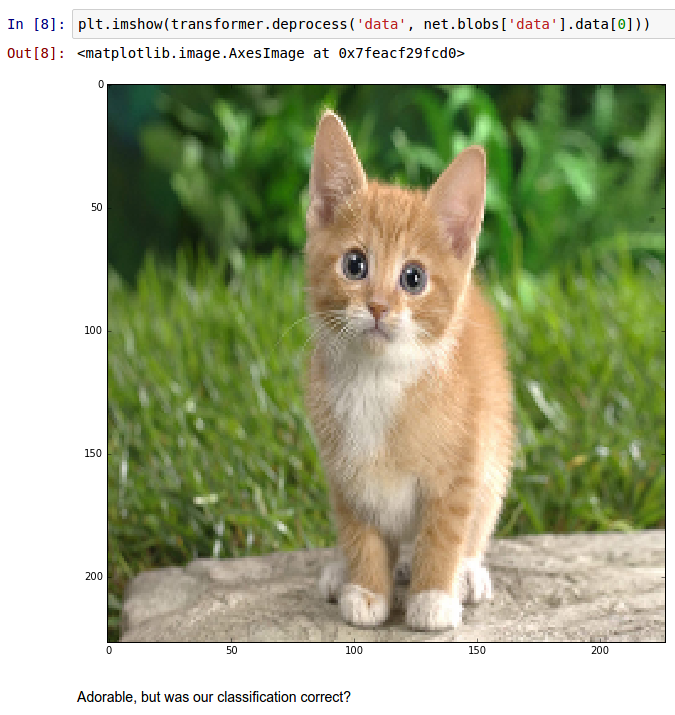
\includegraphics[scale=0.5]{cat.png}

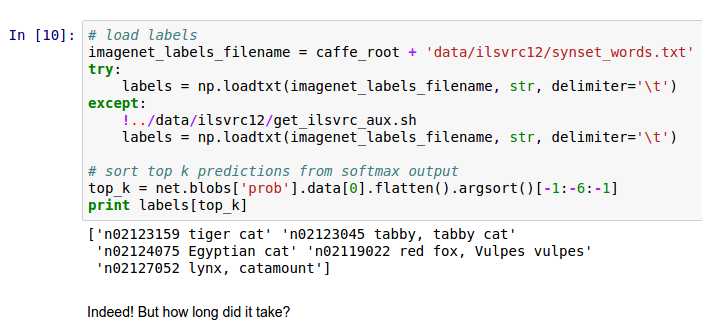
\includegraphics[scale=0.5]{cat2.png}

In the above classification of the cat from the assignment, you can see, that the classifier correctly guesses it is a cat (of some kind). All five guesses are cats (except for the fox, but I'll let it slide).

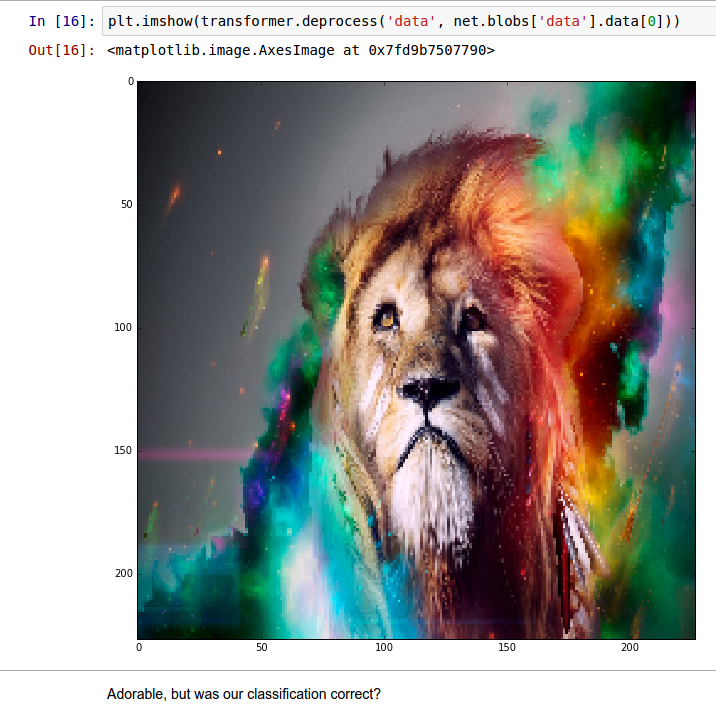
\includegraphics[scale=0.5]{lion1.png}

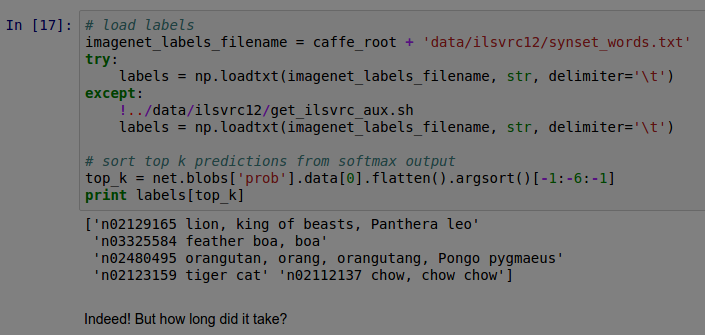
\includegraphics[scale=0.5]{lion2.png}

In the above classification, where we uploaded our own image, you can see, that the classifier correctly guesses a Lion. The next 3 guesses are off, and the fifth guess is somewhat okay. There will be a larger error margin, since the uploaded image is highly photoshopped and abstract.


\section{Week 11: Feature Hashing and LSH}


\end{document}
